% --- IMPORTS ---
\documentclass[leqno]{article}
\usepackage{graphicx}
\usepackage{dsfont}
\usepackage{mathtools}
\usepackage{amssymb}
\usepackage{amsmath}
\usepackage{amsthm}
\usepackage{float}
\usepackage{ragged2e}
\usepackage{tensor}
\usepackage{fancyhdr}
\usepackage{empheq}
\usepackage[most]{tcolorbox}
\usepackage{enumitem}
\usepackage{dirtytalk}
\usepackage{marginnote}
\usepackage{microtype}
\usepackage[
  a4paper,
  left=0.8in,
  right=1in,
  top=1in,
  bottom=0.5in,
  headheight=14pt,
  headsep=0.4in
]{geometry}
\setlength{\parindent}{0cm}
% --- TikZ Packages ---
\usepackage{pgfplots}
\pgfplotsset{compat=1.18}
\usepgfplotslibrary{fillbetween, polar}
\usetikzlibrary{calc, positioning}
\usetikzlibrary{angles, quotes}
\usetikzlibrary{arrows.meta}
\usetikzlibrary{decorations.pathreplacing, decorations.markings}
\usetikzlibrary{patterns}
\usetikzlibrary{intersections}
% --- URL Packages ---
\usepackage[colorlinks=true,linkcolor=red,citecolor=magenta,urlcolor=black]{hyperref}%
\urlstyle{same}
% --- END OF IMPORTS ---

% --- CUSTOM COMMANDS ---
\RenewDocumentCommand{\marks}{o m}{%
  \IfValueTF{#1}%
    {\marginnote{\raggedright\textbf{[#2]}}[#1]}%
    {\marginnote{\raggedright\textbf{[#2]}}}%
}
\newcommand{\vspacerule}[2]{%
  \par\vspace*{#1}%
  \noindent\hrulefill\par
  \vspace*{#2}%
}
\definecolor{scarlet}{RGB}{205, 40, 75}
\newcommand{\questionitem}{%
  \item\phantomsection
  \addcontentsline{toc}{section}{Question \number\value{enumi}}%
}
\renewcommand{\contentsname}{Questions}
% --- END OF CUSTOM COMMANDS ---

% --- HEADER CONFIG ---
\pagestyle{fancy}
\fancyhead{}
\fancyfoot{}
\renewcommand{\headrulewidth}{0.9pt}
\lhead{Complex Roots and Geometry Problems}
\chead{}
\rhead{\href{https://danieljsmith.org}{danieljsmith.org}}
% --- END OF HEADER CONFIG ---

\begin{document}
\vspace*{20pt}
\tableofcontents
\newpage
\begin{enumerate}[
  label=\textbf{\arabic*.},
  leftmargin=*,
  topsep=0pt,
  partopsep=0pt,
  parsep=0pt
]

% ---- Question 1 ----
\questionitem
% [Source: _QBT__Complex_Roots_and_Geometry_Problems, Q1]

\begin{figure}[H]
    \centering
\begin{tikzpicture}[scale=1.2]
\coordinate (O) at (0, 0);
\coordinate (A) at (1.6, 1.6);

\draw[thick, -{Stealth[length=3mm]}] (-3.2, 0) -- (3.6, 0) node[right] {$\mathrm{Re}(z)$};
\draw[thick, -{Stealth[length=3mm]}] (0, -3.2) -- (0, 3.6) node[above] {$\mathrm{Im}(z)$};

\draw[thick] ($(A)+(-0.06,0)$) -- ($(A)+(0.06,0)$);
\draw[thick] ($(A)+(0,-0.06)$) -- ($(A)+(0,0.06)$);

\node[below left] at (O) {$O$};
\node[above right] at (A) {$A$};

\end{tikzpicture}
\end{figure}


An Argand diagram with the point $A$ representing a complex number $z_1$ is shown in the diagram. \\
The complex numbers $z_2$, $z_3$ and $z_4$ are $z_1e^{\frac{1}{2}\pi\mathrm{i}}$, $z_1e^{\pi\mathrm{i}}$ and $z_1e^{\frac{3}{2}\pi\mathrm{i}}$ respectively. \\
\begin{enumerate}[label=\textbf{(\alph*)}]
  \item
  \begin{enumerate}[label=(\roman*)]
    \item On a copy of the Argand diagram, mark the points $B$, $C$ and $D$ representing the complex numbers $z_2$, $z_3$ and $z_4$. \marks[-10pt]{2}
    \item Show that $z_1+z_2+z_3+z_4=0$. \marks{2} \\
  \end{enumerate}
  \item Given now that $z_1$, $z_2$, $z_3$ and $z_4$ are roots of the equation $z^4=-16$, find these four roots, giving your answers in the form $a+\mathrm{i}b$, where $a$ and $b$ are real and exact. \marks{4} \\
\end{enumerate}

\newpage

% ---- Question 2 ----
\questionitem
% [Source: _QBT__Complex_Roots_and_Geometry_Problems, Q2]

The five solutions of the equation $z^5=16+16\sqrt{3}\,\mathrm{i}$ are represented by points on an Argand diagram. \\

These points are the vertices of a regular pentagon $P$ with centre at the origin. \\

\begin{enumerate}
    \item Determine the five complex numbers that represent these vertices, giving your answers in the form $re^{\mathrm{i}\theta}$, where $0\leq \theta<2\pi$. \marks{4} \\

    \item Sketch $P$ on an Argand Diagram, taking care to label each vertex. \marks{2}\\

    \item Show that the area of $P$ can be written $k\sin\frac{2\pi}{5} $ where $k$ is an integer to be determined. \marks{4}
    
\end{enumerate}


\newpage

% ---- Question 3 ----
\questionitem
% [Source: _QBT__Complex_Roots_and_Geometry_Problems, Q3]

\begin{enumerate}[label=(\roman*)]
  \item Find the $8$th roots of $-128+128\sqrt{3}\,\mathrm{i}$ in the form $re^{\mathrm{i}\theta}$, where $r>0$ and $0\leq \theta<2\pi$. \marks{5} \\
  \item These $8$th roots are represented in the Argand diagram, in order of increasing $\theta$, by the points $A$, $B$, $C$, $D$, $E$, $F$, $G$, $H$. \\
  Draw the Argand diagram, making clear which point is which. \marks{2} \\
  \item The mid-point of $BD$ is the point $P$ which represents the complex number $w$. \\
  Find, in exact form, the modulus and argument of $w$. \marks{3} \\
  \item $w$ is an $n$th root of a real number $a$, where $n$ is a positive integer. State the least possible value of $n$ and find the corresponding value of $a$. \marks{3} \\
\end{enumerate}

\newpage


\newpage
% ---- Question 4 ----
\questionitem
% [Source: _QBT__Complex_Roots_and_Geometry_Problems, Q4]

Given that $z_1=7-\mathrm{i}$ and $z_2=\dfrac{z_1}{1-\mathrm{i}}$, \\
\begin{enumerate}[label=\textbf{(\alph*)}]
  \item find $z_2$ in the form $a+b\mathrm{i}$, where $a$ and $b$ are real. \marks{2} \\
  \item Show on an Argand diagram the point $P$ representing $z_1$ and the point $Q$ representing $z_2$. \marks{2} \\
  \item Given that $O$ is the origin, show that $\angle OQP=\dfrac{\pi}{2}$. \marks{2} \\
\end{enumerate}
The circle passing through the points $O$, $P$ and $Q$ has centre $C$. Find \\
\begin{enumerate}[label=\textbf{(\alph*)}, resume]
  \item the complex number represented by $C$. \marks{2} \\
  \item the exact value of the radius of the circle. \marks{2} \\
\end{enumerate}

\newpage

% ---- Question 5 ----
\questionitem
% [Source: _QBT__Complex_Roots_and_Geometry_Problems, Q5]

\begin{figure}[H]
    \centering
\begin{tikzpicture}[scale=1.5]
\def\rad{2}
\coordinate (O) at (0,0);
\coordinate (A) at (\rad,0);
\coordinate (B) at (120:\rad);
\coordinate (C) at (240:\rad);
\coordinate (P) at ({3*\rad},0);
\coordinate (Q) at ({1.5*\rad},{sqrt(3)*\rad/2});
\coordinate (R) at ({1.5*\rad},{-sqrt(3)*\rad/2});
\draw[-{Stealth[length=3mm]}, thick] ({-0.9*\rad},0) -- ({3.35*\rad},0) node[right] {$\mathrm{Re}(z)$};
\draw[-{Stealth[length=3mm]}, thick] (0,{-1.2*\rad}) -- (0,{1.2*\rad}) node[above] {$\mathrm{Im}(z)$};
\draw[thick] (A) -- (B) -- (C) -- cycle;
\draw[thick] (P) -- (Q) -- (R) -- cycle;
\node[below] at (A) {$A$};
\node[above left] at (B) {$B$};
\node[below left] at (C) {$C$};
\node[below] at (P) {$P$};
\node[above right] at (Q) {$Q$};
\node[below right] at (R) {$R$};
\node[below left] at (O) {$O$};
\end{tikzpicture}
\end{figure}


The cube roots of unity are represented on the Argand diagram below by the points $A$, $B$ and $C$. \\

The complex numbers represented by $P$, $Q$ and $R$ are obtained by adding $2$ to the complex numbers represented by $A$, $B$ and $C$ respectively. \\

Determine a degree $6$ polynomial equation with integer coefficients whose roots are the complex numbers represented by the points $A$, $B$, $C$, $P$, $Q$ and $R$. \marks{5}


\newpage

% ---- Question 6 ----
\questionitem
% [Source: _QBT__Complex_Roots_and_Geometry_Problems, Q6]

In an Argand diagram, the points $A$, $B$ and $C$ are the vertices of an equilateral triangle with centre $G$. The point $G$ represents the complex number $1-2\mathrm{i}$, and the point $A$ represents the complex number $5+2\mathrm{i}$. \\
\begin{enumerate}[label=\textbf{(\alph*)}]
  \item Find the complex numbers represented by the points $B$ and $C$, giving your answers in the form $x+\mathrm{i}y$, where $x$ and $y$ are real and exact. \marks{6} \\
\end{enumerate}
The points $D$, $E$ and $F$ are the centroids of triangles $GBC$, $GCA$ and $GAB$ respectively. \\
\begin{enumerate}[label=\textbf{(\alph*)}, resume]
  \item Find the exact area of triangle $DEF$. \marks{4} \\
\end{enumerate}

\newpage

% ---- Question 7 ----
\questionitem
% [Source: _QBT__Complex_Roots_and_Geometry_Problems, Q7]

\begin{figure}[H]
    \centering
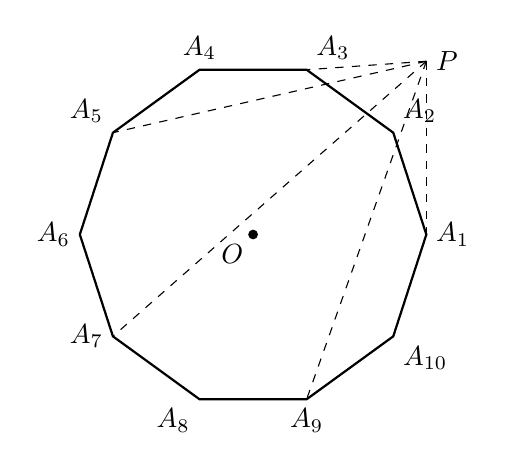
\begin{tikzpicture}[scale=2.2]
\def\R{1}
\pgfmathsetmacro{\step}{360/10}

\coordinate (O) at (0,0);
\coordinate (P) at (1,1);

\foreach \k/\name in {0/A1,1/A2,2/A3,3/A4,4/A5,5/A6,6/A7,7/A8,8/A9,9/A10}{
  \coordinate (\name) at ({\k*\step}:\R);
}

\draw[thick] (A1) -- (A2) -- (A3) -- (A4) -- (A5) -- (A6) -- (A7) -- (A8) -- (A9) -- (A10) -- cycle;

\foreach \Q in {A1,A3,A5,A7,A9}{
  \draw[dashed] (P) -- (\Q);
}

\fill (O) circle[radius=0.8pt];
\node[below left] at (O) {$O$};
\node[right] at (P) {$P$};
\node[right] at (A1) {$A_1$};
\node[above right] at (A2) {$A_2$};
\node[above right] at (A3) {$A_3$};
\node[above] at (A4) {$A_4$};
\node[above left] at (A5) {$A_5$};
\node[left] at (A6) {$A_6$};
\node[left] at (A7) {$A_7$};
\node[below left] at (A8) {$A_8$};
\node[below] at (A9) {$A_9$};
\node[below right] at (A10) {$A_{10}$};
\end{tikzpicture}
\end{figure}


\begin{enumerate}[label=\textbf{(\alph*)}]
  \item Using the identity $zz^*=|z|^2$, or otherwise, show that if $w$ is any root of unity then
  \[
  |w-(1+\mathrm{i})|^2=3-(1-\mathrm{i})w-(1+\mathrm{i})w^*
  \]
  \marks[-20pt]{3}
\end{enumerate}
The diagram shows a regular decagon $A_1A_2\ldots A_{10}$ whose vertices all lie on the unit circle with centre at the origin $O$ and $A_1$ at $(1,0)$. The point $P$ lies in the same plane as the decagon and has coordinates $(1,1)$. \\

\begin{enumerate}[label=\textbf{(\alph*)}, resume]
  \item Using the result from part (a), find
\[
\sum_{r=1}^{5}(PA_{2r-1})^2
\]\marks[-20pt]{4}
\end{enumerate}

\newpage


% ---- Question 8 ----
\questionitem
% [Source: _QBT__Complex_Roots_and_Geometry_Problems, Q8]

You are given the complex number $\alpha=\cos \frac{3\pi}{5}+\mathrm{i}\sin \frac{3\pi}{5}$ and the equation $z^5=-1$. \\
\begin{enumerate}[label=\textbf{(\alph*)}]
  \item Show that $\alpha$ is a root of the equation. \marks{2} \\
  \item Write down the other four roots of the equation. \marks{1} \\
  \item Show that
  \[
  \alpha^4-\alpha^3+\alpha^2-\alpha+1=0
  \]
  \marks[-20pt]{2}
  \item Hence show that
  \[
  \left(\alpha+\frac{1}{\alpha}\right)^2-\left(\alpha+\frac{1}{\alpha}\right)-1=0
  \]
  \marks[-30pt]{3}
  \item Hence determine the value of $\cos \frac{3\pi}{5}$ in the form $a+b\sqrt{c}$, where $a$, $b$ and $c$ are rational numbers to be found. \marks{4} \\
\end{enumerate}

\newpage

% ---- Question 9 ----
\questionitem
% [Source: _QBT__Complex_Roots_and_Geometry_Problems, Q9]

The points representing the complex numbers $z_1=6+11\mathrm{i}$ and $z_2=-8-3\mathrm{i}$ are opposite vertices of a regular octagon, $K$, in the complex plane. \\
The centre of $K$ represents the complex number $\alpha$. \\
\begin{enumerate}[label=\textbf{(\alph*)}]
  \item Show that $\alpha=-1+4\mathrm{i}$. \marks{2} \\
\end{enumerate}
Given that
\[
\beta=\frac{1-\mathrm{i}}{14}
\]
\begin{enumerate}[label=\textbf{(\alph*)}, resume]
  \item Show that
  \[
  \beta(z_1-\alpha)=1
  \]
  \marks[-20pt]{2}
\end{enumerate}
The vertices of $K$ are given by the roots of the equation
\[
(\beta(z-\alpha))^8=1
\]
\begin{enumerate}[label=\textbf{(\alph*)}, resume]
  \item
  \begin{enumerate}[label=(\roman*)]
    \item Write down the roots of the equation $w^8=1$ in the form $re^{\mathrm{i}\theta}$. \marks{1}
    \item Hence, or otherwise, determine the positions of the other six vertices of $K$, giving your answers as complex numbers in Cartesian form. \marks{4} \\
  \end{enumerate}
\end{enumerate}

\newpage


% ---- Question 10 ----
\questionitem
% [Source: _QBT__Complex_Roots_and_Geometry_Problems, Q10]

In an Argand diagram, the points $A$ and $B$ are represented by the complex numbers $1+4\mathrm{i}$ and $7+2\mathrm{i}$ respectively. The circle $C$ passes through $A$ and $B$, and its centre lies on the real axis. \\
\begin{enumerate}[label=\textbf{(\alph*)}]
  \item Find the equation of $C$, giving your answer in the form
  \[
  |z-a|=b \qquad a\in\mathbb{C},\ b\in\mathbb{R}
  \]
  \marks[-20pt]{4}
\end{enumerate}
The circle $D$, with equation $|z-(1+\mathrm{i})|=5$, intersects $C$ at the points representing the complex numbers $z_1$ and $z_2$. \\
\begin{enumerate}[label=\textbf{(\alph*)}, resume]
  \item Find the complex numbers $z_1$ and $z_2$. \marks{5} \\
\end{enumerate}

\newpage


% ---- Question 11 ----
\questionitem
% [Source: _QBT__Complex_Roots_and_Geometry_Problems, Q11]

The cubic equation
\[
z^3+pz^2+qz+24=0
\]
where $p$ and $q$ are real, has roots $\alpha$, $\beta$ and $\gamma$. \\
It is given that $\alpha=-2+2\mathrm{i}$. \\
\begin{enumerate}[label=\textbf{(\alph*)}]
  \item
  \begin{enumerate}[label=(\roman*)]
    \item Write down another root, $\beta$, of the equation. \marks{1}
    \item Find the third root, $\gamma$. \marks{3}
    \item Find the values of $p$ and $q$. \marks{3} \\
  \end{enumerate}
  \item
  \begin{enumerate}[label=(\roman*)]
    \item Express $\alpha$ in the form $re^{\mathrm{i}\theta}$, where $r>0$ and $-\pi<\theta\leq \pi$. \marks{2}
    \item Hence show that
    \[
    (-2+2\mathrm{i})^n=(2\sqrt{2})^n\left(\cos \frac{3n\pi}{4}+\mathrm{i}\sin \frac{3n\pi}{4}\right)
    \]
    \marks[-30pt]{2}
    \item Hence show that
    \[
    \alpha^n+\beta^n+\gamma^n=2(2\sqrt{2})^n\cos \frac{3n\pi}{4}+(-3)^n
    \]
    where $n$ is an integer. \marks{3}
  \end{enumerate}
\end{enumerate}

\newpage

% ---- Question 12 ----
\questionitem
% [Source: _QBT__Complex_Roots_and_Geometry_Problems, Q12]

\begin{figure}[H]
    \centering
\begin{tikzpicture}[scale=1]
\def\rad{3}
\def\rot{30}
\coordinate (O) at (0, 0);
\foreach \k/\lbl in {0/A, 1/B, 2/C, 3/D, 4/E, 5/F} {
  \coordinate (\lbl) at ({\rot + 60*\k}:\rad);
}

\draw[-{Stealth[length=3mm]}, thick] (-3.8, 0) -- (3.8, 0) node[right] {$\mathrm{Re}$};
\draw[-{Stealth[length=3mm]}, thick] (0, -3.8) -- (0, 3.8) node[above] {$\mathrm{Im}$};
\draw[thick] (A) -- (B) -- (C) -- (D) -- (E) -- (F) -- cycle;

\node[below left] at (O) {$O$};
\node[right] at (A) {$A$};
\node[above right] at (B) {$B$};
\node[above left] at (C) {$C$};
\node[below left] at (D) {$D$};
\node[below left] at (E) {$E$};
\node[below right] at (F) {$F$};
\end{tikzpicture}
\end{figure}


In the diagram, the points $A$, $B$, $C$, $D$, $E$ and $F$ represent the complex sixth roots of $-729$ on an Argand diagram. The centroids of triangles $OAB$, $OBC$, $OCD$, $ODE$, $OEF$ and $OFA$ are $G$, $H$, $I$, $J$, $K$ and $L$ respectively. \\
\begin{enumerate}[label=\textbf{(\alph*)}]
  \item Write down, in exponential form, the complex numbers represented by the points $A$, $B$, $C$, $D$, $E$ and $F$. \marks{2} \\
  \item When these complex numbers are multiplied by the complex number $w$, the resulting complex numbers are represented by the points $G$, $H$, $I$, $J$, $K$ and $L$. \\
  Find $w$ in exponential form. \marks{4} \\
  \item You are given that $G$, $H$, $I$, $J$, $K$ and $L$ represent roots of the equation $z^6=p$. \\
  Find $p$. \marks{2} \\
\end{enumerate}


\newpage


% ---- Question 13 ----
\questionitem
% [Source: _QBT__Complex_Roots_and_Geometry_Problems, Q13]

\begin{enumerate}[label=(\roman*)]
  \item Write down, in any form, all the complex roots of the equation
  \[
  w^{11}=-1
  \]
  \marks[-20pt]{2}
  \item Explain why the equation
  \[
  (z+1)^{11}=-(z-1)^{11}
  \]
  has exactly $10$ non-real roots and show that they may be expressed in the form
  \[
  -\mathrm{i}\cot\left(\frac{m\pi}{22}\right)
  \]
  where $m=\pm 1$, $\pm 3$, $\pm 5$, $\pm 7$, $\pm 9$. \marks[-20pt]{6}
  \item Show that
  \[
  \left\{-\mathrm{i}\cot\left(\frac{m\pi}{22}\right)\right\}\left\{\mathrm{i}\cot\left(\frac{m\pi}{22}\right)\right\}=\cot^2\left(\frac{m\pi}{22}\right)
  \]
  \marks[-20pt]{1}
  \item Given that the product of the non-zero roots of the equation in part (ii) is $11$, find the value of
  \[
  \tan^2\left(\frac{\pi}{22}\right)\tan^2\left(\frac{3\pi}{22}\right)\tan^2\left(\frac{5\pi}{22}\right)\tan^2\left(\frac{7\pi}{22}\right)\tan^2\left(\frac{9\pi}{22}\right)
  \]
  \marks[-20pt]{2}
\end{enumerate}
\end{enumerate}
\end{document}
